\documentclass[12pt]{article}

\usepackage[margin=1in]{geometry}
\usepackage{amsmath,amsthm,amssymb}
\usepackage{tikz} % for drawing stuff
\usepackage{xcolor} % for \textcolor{}
\usepackage{readarray} % for \getargsC{}
\usepackage{graphicx} % disjoint union
\usepackage[utf8]{inputenc}
\usepackage[T1]{fontenc}
\usepackage{hyperref}


% Math sets
\newcommand{\N}{\mathbb{N}}
\newcommand{\Z}{\mathbb{Z}}
\newcommand{\R}{\mathbb{R}}

% Setup of project
\newenvironment{question}[2][Question]{\begin{trivlist}
\item[\hskip \labelsep {\bfseries #1}\hskip \labelsep {\bfseries #2.}]}{\end{trivlist}}
\newenvironment{answer}[2][Answer]{\begin{trivlist}
\item[\hskip \labelsep {\bfseries #1}\hskip \labelsep {\bfseries #2:}]}{\end{trivlist}}
\begin{document}
% math enumerate
\renewcommand{\theenumi}{\roman{enumi}}

% Short hands
\let\oldsum\sum
\renewcommand{\sum}[3]{\oldsum\limits_{#1}^{#2}#3}
\let\oldprod\prod
\renewcommand{\prod}[3]{\oldprod\limits_{#1}^{#2}#3}


\title{Homework 2}
\author{Haukur Páll Jónsson\\
NLP 2017}

\maketitle

\begin{question}{1}
Chomsky Normal Form (CNF)
\end{question}
\begin{answer}{a)}{}

The converted grammar is:
\begin{align*}
&S \to NP \text{  } VP \\
&S \to I\_VP \text{  } PP. \text{ We make the rule binary}\\
&I\_VP \to I \text{  } VP \\
&I \to i. \text{ When we make terminal symbols we do not make non-terminal symbols}\\
&NP \to Det \text{  } N\\
&VP \to V \text{  } NP. \text{ We use the fact that }V \to ate \text{ instead of creating a new rule which does exactly the same}\\
&VP \to ate. \text{ We eliminate unit rules}\\
&PP \to Pre \text{  } NP\\
&V \to ate\\
&Det \to the \text{ | }a\\
&N \to fork \text{ | }salad\\
&Pre \to with\\
\end{align*}
\end{answer}

\begin{question}{2}
PCFGs and the CYK algorithm
\end{question}

\begin{answer}{a)}

For any given parse, we compute the probability of that parse by; $p(rule)*p(element\, of \, rule)*p(element \, of \, rule)$
Lets start with the cell marked B: \\
$VP \to V \, Obj \, Obj$, we get: 0.3*0.6*0.2*0.175=0.0063 \\
$VP \to V \, Obj$, we get: 0.5*0.6*0.175=0.0525 \\
$VP \to V \, small$, we get: 0.2*0.6*0.08=0.0096 \\

For the cell marked A we essentially get all of the probabilities of B times 0.3: \\
$S \to Subj \, VP$, we get: 1.0*0.3*0.0063=0,00189 \\
$S \to Subj \, VP$, we get: 1.0*0.3*0.0525=0,01575 \\
$S \to Subj \, VP$, we get: 1.0*0.3*0.0096=0.00288 \\

%\begin{table}[]
%\centering
%\caption{My caption}
%\label{my-label}
%\begin{tabular}{|l|l|l|l|l|}
%\hline
%     & I                 & make              & her                                                                                    & duck                                                                                                                                                                                                              \\ \hline
%I    & $Subj \to I$, 0.3 & -                 & \begin{tabular}[c]{@{}l@{}}$S \to Subj VP$,\\   1.0*0.3*0.06\end{tabular}              & \begin{tabular}[c]{@{}l@{}}$S \to Subj VP$,\\   1.0*0.3*0.0063=0,00189\\ $S \to Subj VP$,\\   1.0*0.3*0.0525=0,01575\\ $S \to Subj VP$,\\   1.0*0.3*0.0096=0.00288\end{tabular}                                   \\ \hline
%make &                   & $V \to make$, 0.6 & \begin{tabular}[c]{@{}l@{}}$VP \to V \medskip Obj$, \\   0.5*0.6*0.2=0.06\end{tabular} & \begin{tabular}[c]{@{}l@{}}$VP \ to V Obj Obj$, \\   0.3*0.6*0.2*0.175=0.0063\\ $VP \to V Obj$,\\   0.5*0.6*0.175=0.0525\\ $VP \to V small$,\\   0.2*0.6*0.08=0.0096\end{tabular}                                 \\ \hline
%her  &                   &                   & \begin{tabular}[c]{@{}l@{}}$Obj \to her$, 0.2\\ $Det \to her$, 1.0\end{tabular}        & \begin{tabular}[c]{@{}l@{}}$small \to Obj \medskip V$, \\   1.0*0.2*0.4=0.08\\ $NP \to Det \medskip N$, \\   0.5*1.0*0.5=0.25\\ $Subj \to NP$, \\   0.8*0.25=0.2\\ $Obj \to NP$, \\   0.7*0.25=0.175\end{tabular} \\ \hline
%duck &                   &                   &                                                                                        & \begin{tabular}[c]{@{}l@{}}$V \to duck$, 0.4\\ $N \to duck$, 0.5\\ $NP \to N$, 0.5*0.5=0.25\\ $Subj \to NP$, 0.8*0.25=0.2\\ $Obj \to NP$, 0.7*0.25=0.175\end{tabular}                                             \\ \hline
%\end{tabular}
%\end{table}
\end{answer}
\begin{answer}{b)}

  The most probable parse:

  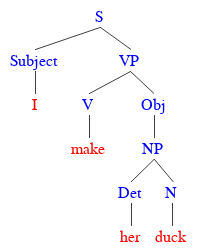
\includegraphics[scale=0.5]{tree}
  %In bracket notation the most probable parse is:
  %[S [Subject I] [VP [V make]  [Obj [NP [Det her] [N duck]] ]]]

\end{answer}

\begin{question}{3}
Dependency parsing /MST
\end{question}

\begin{answer}{a)}{CLE}


\end{answer}

\begin{answer}{b)}{Final step}


\end{answer}

\begin{question}{4}
Dependency parsing / Transistion based
\end{question}

\begin{answer}{a)}{Arc-standard system}


\end{answer}
\end{document}
